% !TeX document-id = {627414bf-e7a2-4218-9269-f76848e4211f}
%%
%% F5 compiles the whole document, runs bibliography, etc
%% F6 compiles the document only once, tableofcontents may be not correct after running this
%% F8 run biber
%%
% !TeX program = lualatex
% !TeX TXS-program:quick = txs:///lualatex/[--shell-escape] | txs:///biber | txs:///lualatex/[--shell-escape] | txs:///lualatex/[--shell-escape] | txs:///view
% !TeX TXS-program:compile = txs:///lualatex/[--shell-escape] | txs:///view
% !BIB program = biber
% !TeX encoding = utf8
% !TeX spellcheck = de_DE
% !TeX root = thesis.tex

\documentclass[
english,
%german,
%standalone,
%final,
]{bama}

%Authors firstname, put a space behind the name
\firstname{Manfred }

%Authors lastname
\lastname{Mustermann}

%Type of thesis (Bachelorarbeit, Masterarbeit, Bachelor's Thesis, Master's Thesis)
\thesis{Bachelorarbeit}

%Course, EEI/IuK/MT/...
\course{Elektrotechnik, Elektronik und Informationstechnik (EEI)}

%Title of the work
\title{Ein sehr sehr langer Titel, der mehrere Zeilen umspannt, wie sie bei Abschlussarbeiten häufiger vorkommen}
\subtitle{Untertitel der Arbeit}

%Keywords saved in the metadata, put something like FPGA, SCPI, RADAR, ... (separate with ;)
\keywords{keyword1; keyword2}

%Names of tutors/Betreuer/supervisors including titles (seperate with ;)
%Corresponding professor
	%Prof. Dr.-Ing. Dr.-Ing. habil. Robert Weigel
	%Prof. Dr.-Ing. Georg Fischer
%team leader and/or group leader if primary tutor is not Akademischer Rat*in
	%https://www.lte.tf.fau.de/lehrstuhl/person/
%primary tutor
\supervisor{Betreuer 1; Betreuer 2; Betreuer 3; Betreuer 4} %seperate with ;

%Begin date of thesis (format corresponding to the chosen language)
\thesisbegin{01.01.1970}

%Same for the end
\thesisend{09.02.2021}

%Month and year when thesis is handed in
%required for financial stuff at the institute
\thesisendmonth{2} %number of the month without leading 0 (1-12)
\thesisendyear{2021}

%Abstract for pdf metadata. This abstract will be visible in the archive of LTE and is visible in the metadata of the pdf output file. Avoid TeX here.
\abstract{
	Lörem ipsüm dolor sit ämet, consetetur sadipscing elitr, sed diam nonumy eirmod tempor invidunt ut labore et dolore magna aliquyam erat, sed diam voluptua. At vero eos et accusam et justo duo dolores et ea rebum. Stet clita kasd gubergren, no sea takimata sanctus est Lorem ipsum dolor sit amet. Lorem ipsum dolor sit amet, consetetur sadipscing elitr, sed diam nonumy eirmod tempor invidunt ut labore et dolore magna aliquyam erat, sed diam voluptua. At vero eos et accusam et justo duo dolores et ea rebum. Stet clita kasd gubergren, no sea takimata sanctus est Lorem ipsum dolor sit amet. Lorem ipsum dolor sit amet, consetetur sadipscing elitr, sed diam nonumy eirmod tempor invidunt ut labore et dolore magna aliquyam erat, sed diam voluptua. At vero eos et accusam et justo duo dolores et ea rebum. Stet clita kasd gubergren, no sea takimata sanctus est Lorem ipsum dolor sit amet.
	\\
	Duis autem vel eum iriure dolor in hendrerit in vulputate velit esse molestie consequat, vel illum dolore eu feugiat nulla facilisis at vero eros et accumsan et iusto odio dignissim qui blandit praesent luptatum zzril delenit augue duis dolore te feugait nulla facilisi. Lorem ipsum dolor sit amet.
}

%define bibliography file containing references
%edit this file in editor or with tools like jabref
%references can be downloaded at ub.fau.de, ieeexplore.com and via the online tool in jabref, paste in jabref from clipboard is possible
%thesis with modern lte templates can be drag and dropped into jabref
\bibliography{bibliography/bibliography.bib}

%define your acronyms in this file
%defines acronyms of long version used in text
%reference them with \ac{LNA} to get the long version at first use
%more commands see here: https://ctan.org/pkg/acro
\DeclareAcronym{IHD}{
	short = IHD,
	long = Ischemic Heart Disease,
}

\DeclareAcronym{NCDs}{
	short = NCDs,
	long = Noncommunicable Diseases,
}

\DeclareAcronym{AF}{
	short = AF,
	long = Atrial Fibrillation,
}

\DeclareAcronym{AI}{
	short = AI,
	long = Artificial Intelligence,
}

\DeclareAcronym{ADC}{
	short = ADC,
	long = Analog-to-Digital Converter,
}

\DeclareAcronym{IoT}{
	short = IoT,
	long = Internet of Things,
}


\DeclareAcronym{CVD}{
	short = CVD,
	short-plural = s,
	long =  Cardiovascular disease,
}


\DeclareAcronym{ECG}{
	short = ECG,
	long  = Electrocardiogram
}


\DeclareAcronym{FAU}{
	short = FAU,
	long  = Friedrich-Alexander-Universität
}

\DeclareAcronym{MOSFET}{
	short = MOSFET,
	long  = Metal-Oxide-Semi\-conductor Field-Effect Tran\-sistor
}

\DeclareAcronym{FFT}{
	short = FFT,
	long  = Fast Fourier Transformation
}

\DeclareAcronym{LTE}{
	short = LTE,
	long  = Lehrstuhl für Technische Elektronik,
	long-plural-form = Lehrstühle für Technische Elektronik 	% Unnütz, zeigt nur, wie es geht
}

\DeclareAcronym{BA}{
	short = BA,
	short-plural = s,
	long = Bachelorarbeit,
	long-plural = en
}

\DeclareAcronym{MA}{
	short = MA,
	short-plural = s,
	long = Masterarbeit,
	long-plural = en
}

%define manual hyphenation if automatic does not work well
\hyphenation{Dynamik-bereich}

%header with packages for special use cases
% -----------------------------------------

%math stuff
%defines math symbols and fonts
%%% math mode
%%% ---------

\usepackage{mathtools}
\usepackage{unicode-math}
\usepackage{lualatex-math}	% Lädt einige Korrekturen für amsmath, mathtools und weitere.

%math font using unicode-math
\IfFontExistsTF{TeX Gyre Termes Math}{
	\setmathfont{TeX Gyre Termes Math}}{
	\setmathfont{texgyretermes-math.otf}}

%make normal text in math mode look like other text
\IfFontExistsTF{TeX Gyre Termes}{
	\setmathfont{TeX Gyre Termes}[range=\mathup/{latin,Latin,num,greek,Greek}]}{
	\setmathfont{texgyretermes-regular.otf}[range=\mathup/{latin,Latin,num,greek,Greek}]}

%custom mathematical symbols
\AtBeginDocument{%
	%upright partial derivation symbol
	\let\umathpartial\partial
	\renewcommand\partial{\symup\umathpartial}
	
	%upright letters for constants
	\newcommand\jj{\operatorname{j}}
	\newcommand\ii{\operatorname{i}}
	\newcommand\ee{\operatorname{e}}
	\newcommand\pipi{\uppi}
	\let\jmath\jj
	
	%upright integral d
	\newcommand\dd[1]{\,\operatorname{d}\!#1\xspace}
	
	%vector arrow
	\newcommand{\vect}[1]{\overrightarrow{#1}}
	
	%upright grad, div, rot
	\DeclareMathOperator{\grad}{grad}
	\DeclareMathOperator{\diver}{div}
	\DeclareMathOperator{\rot}{rot}
	
	%limits can be used with _ and ^ and are always placed above and unter the int sign
	\let\intold\int
	\removenolimits{\int}\removenolimits{\iint}\removenolimits{\iiint}
	\removenolimits{\oint}\removenolimits{\oiint}\removenolimits{\oiiint}
}

\usepackage{esint}

%numbers and units
\ifgerman{
	\usepackage[locale=DE, per-mode=symbol-or-fraction, detect-all=true]{siunitx}
}
\ifenglish{
	\usepackage[per-mode=symbol-or-fraction, detect-all=true]{siunitx}
}
\usepackage{icomma} %correct spacing in german mode


%code listings
%%% code listings
%%% -------------

% Farben definieren für package listings 
%\usepackage{color}
%\definecolor{middlegray}{rgb}{0.5,0.5,0.5}
%\definecolor{lightgray}{rgb}{0.8,0.8,0.8}
%\definecolor{orange}{rgb}{0.8,0.3,0.3}
%\definecolor{yac}{rgb}{0.6,0.6,0.1}
\definecolor{commentgreen}{rgb}{0,0.6,0.0}
\definecolor{keyred}{RGB}{127,0,85}

% Syntax highlighting
\usepackage{listings}
\usepackage{lstautogobble}
\lstset{
	basicstyle=\small\ttfamily,
	%keywordstyle=\bfseries\ttfamily\color{red},
	stringstyle=\color{purple}\ttfamily,
	commentstyle=\color{teal}\ttfamily, %comments in green
	numberstyle=\color{grey},
	showtabs=false,
	showspaces=false,
	showstringspaces=false,
	flexiblecolumns=false,
	tabsize=2,
	numbers=left, %line numbers
	numberstyle=\tiny,
	numberblanklines=true,
	stepnumber=1,
	numbersep=10pt,
	xleftmargin=15pt,
	breaklines=true, %line breaks
	breakatwhitespace=true,
	autogobble=true, %autoremove indention
} 


%%% figures
%%% -------

\usepackage{float}
\usepackage{wrapfig}
%\usepackage[hyperref=false]{scrhack} %solves komascript incompatibilities
%\usepackage[countmax]{subfloat}
\usepackage[section]{placeins} %ensure figures are in the correct section
%\usepackage[format=hang]{caption}
\usepackage{subcaption} %allow figures with subfigures

% Standardargument für Platzierung von figures und tables kann hier global mit absteigender Priorität eingestellt werden.
% Vorgabe: tbp (1. oben, 2. unten, 3. eigene Seite)
% Weitere Möglichkeiten: h (hier), H (unbedingt hier)
\makeatletter
\renewcommand{\fps@figure}{htbp}
\renewcommand{\fps@table}{htbp}  
\makeatother
% Ende Spezialanpassung figures


%packages for graphics created in LaTeX
%standalone, tikz, pgfplots
%%% Tikz drawings
%%% ------------

\usepackage[mode=tex]{standalone}
%\usepackage[mode=buildnew]{standalone}

\usepackage{tikz}
\usepackage{tikzsymbols}
\usepackage[european,cuteinductors]{circuitikz}
\usetikzlibrary{calc,arrows,patterns}

% pgfplot
\usepackage{pgfplots}
\usepgfplotslibrary{smithchart}
\usepgfplotslibrary{groupplots}

%\pgfplotsset{compat=1.10}
%\pgfplotsset{every tick label/.style={font={\scriptsize}}}
%\pgfplotsset{every axis label/.style={font={\small}}}
%\pgfplotsset{every legend /.style={font={\boldmath\small\bfseries}}}
%\pgfplotsset{every label/.style={font={\boldmath\small\bfseries}}}

\pgfplotsset{width=.8\textwidth}
\pgfplotsset{height=.5\textwidth}
\pgfplotsset{grid=both}
\pgfplotsset{major tick style={thin,black}}% modifies the style ‘every tick’
\pgfplotsset{minor tick style={very thin,black}}% modifies the style ‘every tick’
\pgfplotsset{major grid style={thin}} %modifies the style ‘every major grid’
\pgfplotsset{minor grid style={very thin}} % modifies the style ‘every minor tick’
%\pgfplotsset{minor x tick num=1} %n minor ticks zwischen major ticks(major tiks müssen selben abstand haben) (problems with smithchart)
%\pgfplotsset{minor y tick num=1} %n minor ticks zwischen major ticks(major tiks müssen selben abstand haben) (problems with smithchart)
%\pgfplotsset{xlabel near ticks,ylabel near ticks}
%For ylabel offsets:

%For ylabel offsets:
\pgfplotsset{ylabsh/.style={every axis y label/.style={at={(0,0.5)}, xshift=#1, rotate=90}}}
\pgfplotsset{xlabsh/.style={every axis x label/.style={at={(0.5,0)}, yshift=#1}}}
\pgfplotsset{filter discard warning=false}%disable filter warning using "each nth point"

\pgfplotsset{every axis/.append style={line width=1pt}}

%cycle list für plots, !!!! \addplot+ verwenden!
%\pgfplotsset{
%	cycle list={
%		blue,
%		red,
%		{black, thick, dashed},
%		violet
%	}
%} 


\begin{document}
	%roman page numbering, etc..	
	\frontmatter
	
	%title page
	\maketitle

	%declaration of own work...
	\declaration

	%summary of the work
	%(not as much result orientated as the summary at the end)
	% !TeX root = ../thesis.tex

%German abstract, optional for thesis written in english
\ifgerman{
	\chapter*{Kurzfassung}
	\label{sec:kurzfassung}

	Lorem ipsum dolor sit amet, consetetur sadipscing elitr, sed diam nonumy eirmod tempor invidunt ut labore et dolore magna aliquyam erat, sed diam voluptua. At vero eos et accusam et justo duo dolores et ea rebum. Stet clita kasd gubergren, no sea takimata sanctus est Lorem ipsum dolor sit amet. Lorem ipsum dolor sit amet, consetetur sadipscing elitr, sed diam nonumy eirmod tempor invidunt ut labore et dolore magna aliquyam erat, sed diam voluptua. At vero eos et accusam et justo duo dolores et ea rebum. Stet clita kasd gubergren, no sea takimata sanctus est Lorem ipsum dolor sit amet. Lorem ipsum dolor sit amet, consetetur sadipscing elitr, sed diam nonumy eirmod tempor invidunt ut labore et dolore magna aliquyam erat, sed diam voluptua. At vero eos et accusam et justo duo dolores et ea rebum. Stet clita kasd gubergren, no sea takimata sanctus est Lorem ipsum dolor sit amet.

	Duis autem vel eum iriure dolor in hendrerit in vulputate velit esse molestie consequat, vel illum dolore eu feugiat nulla facilisis at vero eros et accumsan et iusto odio dignissim qui blandit praesent luptatum zzril delenit augue duis dolore te feugait nulla facilisi. Lorem ipsum dolor sit amet.
}

% English abstract, required for german and english thesis language
\chapter*{Abstract}
\label{sec:abstract}

Ischemic heart diseases are currently a leading cause of mortality worldwide, responsible for approximately 16\% of total global deaths. This underscores the importance of timely detection of heart rate variabilities in reducing mortality rates. Current techniques for detecting heart rate variabilities involve extracting RAW ECG data and transmitting it to remote or cloud servers for further analysis. However, this approach is inconvenient for continuous monitoring as it results in significant power consumption.

\vspace{1em}

\noindent Over the past decade, the \ac{IoT} has become increasingly integrated into our daily lives. Everything from TVs, speakers, and toys, to appliances is now connected to the internet. With the rapid increase in \ac{IoT} data and the emergence of AI, there's an opportunity for edge intelligence. Integrating edge AI with IoT can bring additional benefits to systems, such as reduced power consumption, lower latency, bandwidth optimization, and enhanced data security.

\vspace{1em}

\noindent Designing an end-to-end device for recording \ac{ECG} and predicting heart rate variability on the edge, while ensuring user data security through encryption, is the focus of this thesis. In this regard, a simple, cost-efficient analog circuit PCB is designed to detect the R-peaks of ECG, and a method for translating and deploying neural network models on embedded devices using MAX78000 APIs is presented. Additionally, a secure element is interfaced with the device to enhance its safety features. 

\vspace{1em}


\noindent The extracted ECG signals are further compared with off-the-shelf ECG Holter monitors in terms of R-peak detection. Furthermore, a comparison is made in terms of power and energy consumption between transmitting ECG raw data to a remote server via Bluetooth and performing edge computation for heart rate variability detection.


	%table of contents including heading
	\tableofcontents
	
	%table with acronyms specified in the acronyms file and used in thesis
	\printacronyms

	%arabic page numbering
	\mainmatter
	
	%demonstration of LaTeX capabilities
	%Introduction to LaTeX
% !TeX root = ../thesis.tex

\chapter{BaMa Template}

\section{\LaTeX~Basics}

LaTeX uses source code which is compiled to generate documents. This has several advantages when creating large documents: 

\begin{itemize}
	\item Separation of template and document possible
	\item Consistent text format across sections and documents oriented at norms like DIN~1450
	\item Customisable and reproducible generation of table of contents, figures and index
	\item Automation of tasks like number formatting, plot generation, \dots
	\item Inclusion of external files like measurement data without the need for copy and paste
	\item Automated tasks like number formatting 
\end{itemize}

\subsection{Command syntax}

LaTeX commands have the following syntax:

\begin{lstlisting}
	\command[options]{argument}
\end{lstlisting}

There are also environments which can be opened and closed:

\begin{lstlisting}
	\begin{environmentname}
		...
	\end{environmentname}
\end{lstlisting}

As the backslash is used as prefix for commands and the percent sign for commands a few escape sequences are necessary as listed in table~\ref{tab:escseq}. For more special characters see \url{http://detexify.kirelabs.org/classify.html}.

\begin{table}[H]
	\centering
	\caption{\LaTeX escape sequences}
	\label{tab:escseq}
	\begin{tabular}{ccc}
		\toprule
		Sign & \LaTeX special meaning  & Escape sequence\\
		\midrule
		\textbackslash~(backslash) & command initializer & \verb|\textbackslash| \\
		\%~(percent) & comment for rest of line & \verb|\%| \\
		\textasciitilde~(tilde) & line break protected space & \verb|\textasciitilde| \\
		\$~(dollar sign) & start math mode & \verb|\$| \\			
		\bottomrule
	\end{tabular}
\end{table}

\subsection{Main document structure}

Documents normally have the following components:

\begin{itemize}
	\item \verb|\documentclass[options]{classname}|: Loads the documents template which defines the appearance like article, conference paper, \dots. The bama template uses a custom class located in the main directory of the repository.
	\item \verb|\usepackage[options]{packagename}|: Loads packages for additional capabilities. More information about packages is available at ctan \footnote{\url{https://www.ctan.org/}}.
	\item \verb|\input{filename}|: Inserts the content of another \TeX file \footnote{include serves a similar purpose, has more restrictions but offers  higher compilation speeds.}.
	\item The content of the document in between \verb|\begin{document}| and \verb|\end{document}|
\end{itemize}

\subsection{Heading structure}

There are several levels of headings which are listed in the following. Avoid having a single heading of a certain hierarchy e.g. if there is section 1.1 there should also be at least 1.2.

\begin{description}
	\item [part] is the highest hierarchy. Parts have big headings occupying a whole page. It is not needed for the thesis.
	\item [chapter] is a high hierarchy heading causing page breaks to next uneven page. It is not available in all classes but should be used for the thesis.
	\item [section] is used to separate chapters. One can also use \verb|\subsection| and \verb|\subsubsection| for further hierarchy levels.
	\item [paragraph] and \verb|\subparagraph| are used for small passages and do not cause a line break after the heading.
\end{description}

\subsection{Text formatting}

LaTeX distinguishes between line break and paragraph. Do not use the line break operator for paragraphs, just insert an empty line in the source code. Sometimes special formatting is useful e.g. to center figures but manual font size and style changes in normal text should be avoided.

\begin{table}[H]
	\centering
	\caption{Text formatting}
	\label{tab:textformat}
	\begin{tabular}{ccc}
		\toprule
		Feature & command\\
		\midrule
		Line break & \verb|\\| \\
		Paragraph & empty line in code \\
		\textit{italic} & \verb|\textit{...}| \\
		\textbf{bold} & \verb|\textbf{...}| \\
		center & \verb|\centering| \\	
		\bottomrule
	\end{tabular}
\end{table}

\subsection{Dashes}

\begin{table}[H]
	\centering
	\caption{Dashes}
	\label{tab:dashes}
	\begin{tabular}{cccc}
		\toprule
		Name & Code & Example & Usage\\
		\midrule
		dash & \verb|-| & - & hyphen\\
		Viertelgeviertstrich & &  & Binde-, Trennungs-, Ergänzungsstrich\\
		en dash & \verb|--| & -- & number range\\
		Halbgeviertstrich & & & Gedanken-, Bis-strich, bei Geldbeträgen\\
		em dash & \verb|---| & --- & parenthetic expression \\
		Geviertstrich &  & & Spiegelstrich\\
		%Doppelgeviertstrich & \verb|--\,--| & --\,-- & Zensurstrich (englisch)
		\bottomrule
	\end{tabular}
\end{table}

Hyphens are automatically inserted to break lines and achieve justification. Although the corresponding parameters should be set correctly special words can lead to problems. For example MUSIC-Alogrithmus has a dash which means that hypens at other places are not allowed. This can be prevented by the syntax \hbox{\verb|MUSIC-Algo\-rithmus|} which allows an optional line break. The same problems can occur due to protected whitespaces.

\subsection{Lists}

There are two major list types in {\LaTeX}: numerated (\texttt{enumerate}) and not numerated (\texttt{itemize}). Furthermore there is the type \texttt{description} for explaining keywords. Lists are started with \texttt{begin} and stopped with \texttt{end}. They can also be nested.

\begin{enumerate}
	\item High level with numbering
	\begin{itemize}
		\item Detailed information
		\item without numeration
	\end{itemize}
	\item Another big point
	\item \dots and more
\end{enumerate}

\begin{lstlisting}[language=TeX]
\begin{enumerate}
	\item High level with numbering
	\begin{itemize}
		\item Detailed information
		\item without numeration
	\end{itemize}
	\item Another big point
	\item \dots and more
\end{enumerate}
\end{lstlisting}

\section{Math mode and Numbers}

	Normaly LaTeX operates in text mode, but for expressions like $x=5$ the math mode can be activated and deactivated using \verb|$|. In math mode text is italic and exhibits changed letter spacing.
	
	For indexed equations the \verb|equation| environment is suited when using vanilla LaTeX. With the package \verb|amsmath| the \verb|align| environment is available which is recommended here:
	
	\begin{align}
		\label{eq:alignDemo}
		\oint_{\partial A} \vect{B}_\text{ind} \dd{\vect{l}} &= \mu_0 \left( \iint_A \vect{j}_\text{ind} \dd{\vect{A}} + \varepsilon_0 \frac{\partial}{\partial t} \iint_A \vect{E} \dd{\vect{A}} \right) \\
		\text{und außerdem} \nonumber \\
		\label{eq:alignDemo2}
		Q &= \oiint_A \vect{D} \dd{\vect{A}} = \iiint_V \rho_{\text{Volumen}} \dd{V}
	\end{align}
	
	\begin{lstlisting}[language=TeX]
	\begin{align}
	\label{eq:alignDemo}
	\oint_{\partial A} \vv*{B}{\text{ind}} \dd{\vv{l}} &=
		\mu_0 \left( \iint_A \vv*{j}{\text{ind}} \dd{\vv{A}}
		+ \varepsilon_0 \frac{\partial}{\partial t} \iint_A \vv{E} \dd{\vv{A}} \right) \\
	\text{und außerdem} \nonumber \\
	\label{eq:alignDemo2}
	Q &= \oiint_A \vv{D} \dd{\vv{A}} = \iiint_V \rho_{\text{Volumen}} \dd{V}
	\end{align}
	\end{lstlisting}

	Equations can be easily referenced when the package \verb|mathtools| is used by the the command \verb|\eqref{eq:alignDemo}| (e.g. Eq.~\eqref{eq:alignDemo}).
	
	Between numbers and units a half length space has to be inserted (\verb|\,|) \footnote{For details see DIN~1338}. In German a comma has to be used instead of a dot. The package \verb|siunitx| can handle the correct formatting of numbers with units. The syntax is showed in table~\ref{tab:numberUnitFormat}. Also note that in German the letter \enquote{$U$} is used for voltage instead of \enquote{$V$}.
	
	\begin{table}
		\centering
		\caption{Number- and Unit formatting}
		\label{tab:numberUnitFormat}
		\begin{longtable}{p{.25\textwidth}p{.1\textwidth}p{.1\textwidth}p{.4\textwidth}}
			\toprule
			Variables & \textit{italic} & $x$\newline $y$\newline $f$\newline $\omega$ & \verb|$x$|\newline \verb|$y$|\newline \verb|$f$|\newline \verb|$\omega$|\\
			Scientific constants & \textit{italic} & $c_0$\newline $\mu_0$\newline $\varepsilon_0$ & \verb|$c_0$|\newline \verb|$\mu_0$|\newline \verb|$\varepsilon_0$|\\
			Units & upright & \si{\milli\ampere}\newline $\SI{3.0}{\micro\metre}$\newline \SI{1.41}{} & \verb|\si{\milli\ampere}|\newline \verb|$\SI{3.0}{\micro\metre}$|\newline \verb|\SI{1.41}{}|\\
			Operators & upright & $\frac{\dd{x}}{\dd{y}}$\newline $\sin$\newline $\cos$\newline $\arg$ & \verb|$\frac{\dd{x}}{\dd{y}}$|\newline \verb|$\sin$|\newline \verb|$\cos$|\newline \verb|$\arg$|\\
			Mathematic constants & upright & $\ee$\newline $\ii$\newline $\jj$\newline $\pipi$ & \verb|$\ee$|\newline \verb|$\ii$|\newline \verb|$\jj$|\newline \verb|$\pipi$| \\
			\bottomrule
		\end{longtable}
	\end{table}

	\section{Floating environments}
	\label{sec:floatenvironments}
	
		Floating objects are objects whose position in the final document can depart from the source code. The most common floating objects are figures and tables. Commonly they are placed at the top or bottom of a page to not split the text apart and make reading more pleasant. Floats can also be longer than a single page.
		
		Floats are created by using \verb|\begin{figure}| / \verb|\end{figure}| for figures and \verb|\begin{table}| / \verb|\end{table}| for tables. The content is defined in between and can be arbitrarily chosen. Floats should have a meaningful caption which is specified with \texttt{{\textbackslash}caption[register entry]\{caption text\}}. The command \texttt{{\textbackslash}label} is used to enable referencing them.
		
		Sometimes {\LaTeX} has troubles to determine the best position for a float. In these cases optional arguments or packages like \texttt{placeins} can be used.
		
		\begin{itemize}
			\item t (top, top of page)
			\item b (bottom, bottom of page)
			\item p (page, on an individual page)
			\item h (here, exactly at this position)
			\item H (HERE, forced to place exactly at this position (provided by the package \texttt{float})
		\end{itemize}
		
		As the options are not enforced one can add a second priority \verb|\begin{figure}[tb]|. The only enforced option is \enquote{H}.

		Instead of forced positioning the float environment can also be skipped and the caption with \texttt{{\textbackslash}captionof\{figure/table\}[register entry]\{caption text\}} added.
		
		\paragraph{Labels and References}
		
		Floating elements are commonly labeled using a \texttt{label} which is issued after the caption. It is recommended to add the type of object e.g. \verb|\label{eq:maxwell}|, \verb|\label{fig:blockDiagramTx}|. Labels can also be created for sections, subsections, \dots.
		The labels can be references using \verb|\ref{fig:blockDiagramTx}|. Only the number is output so you have to add the type manually e.g. \verb|see figure~\ref{fig:blockDiagramTx} and equation~\eqref{eq:maxwell}|. It will look like this figure~\ref{fig:tikz}. The page can be found with \verb|\pageref|. Multiple compilations are required until all references are correctly included in the document.
		
		\paragraph{Caption}
		
		Always choose a meaningful caption for floats, especially if they are not directly placed at the text section. If figures are included from other documents always add a citation to the caption.
	
	\subsection{Figures}
	\label{sec:figures}
	
		\subsubsection{External Graphics}
			
		Graphics can be included using the package \texttt{graphicx} as it is done on the title page. Vector graphics are recommended over pixel graphics. They can be included in the format pdf. The include command is \verb|\includegraphics[width=.8\textwidth]{imagefile}|. Alternatively the height can be specified and also given in cm.
		
		\begin{lstlisting}[language=TeX]
			\begin{figure}[tb]
				\centering
				\includegraphics[width=.8\textwidth]{images/receiverChain}
				\caption{Description and then references \cite{BibDEMO1, BibDEMO2, BibDEMO3}}
				\label{fig:receiverChain}
			\end{figure}
		\end{lstlisting}
	
		\subsubsection{Tikz and Circuitikz}
		
		Tikz is a package based on pgf and allows to draw graphics using lines, rectangles, polygons and so on. There is also a further extension called Circuitikz which allows to draw schematics and also has been enhanced by \acs{LTE}.
		
		There are several approaches to avoid long compilation times when drawing a new graphic:
		
		\begin{itemize}
			\item Develop the graphic using KtikZ resp. QtikZ and paste it into the thesis
			\item Use tikz externalize to save compiled graphics automatically in external files
			\item Use standalone class to create a separate document for the graphic. The {\TeX} is later imported to the main document.
		\end{itemize}
	
		For this template the later option is chosen because it has the additional advantage that graphics can be reused in further documents like papers or presentations. Required packages for the external graphics can be loaded in one of the header files and included in both documents. The filter in Figure~\ref{fig:tikz} is used as an example for this method.
		
		\begin{lstlisting}[language=TeX]
		\begin{figure}
			\centering
			\includestandalone{standalones/filter/filter}
			\caption{Schaltplan einer Operationsverstärkerschaltung, erstellt in circuitikz mit Hilfe der Entwicklungsumgebung QTikZ}
			\label{fig:tikz}
		\end{figure}.
		\end{lstlisting}
		
		\begin{figure}
			\centering
			\includestandalone{standalones/filter/filter}
			\caption{Schaltplan einer Operationsverstärkerschaltung, erstellt in circuitikz mit Hilfe der Entwicklungsumgebung QTikZ}
			\label{fig:tikz}
		\end{figure}
	
		\subsubsection{Styling of Plots}
		
		Plots are a common element of a thesis. In order to achieve high quality plots they can be directly generated using {\TeX} or imported using a suited vector graphic format.
		
		Scientific plots have to be labelled correctly. Only the following formats are allowed. The space before and after \enquote{in} / the slash can vary.
		
		\begin{enumerate}
			\item $E${\qquad}in{\qquad}\si{\volt\per\meter}
			\item $E$ / (\si{\volt}/\si{\meter})
		\end{enumerate}
	
		\subsubsection{pgfplots}
		
		Plots from expressions, measured or simulated data can be directly plotted using the famous \texttt{pgfplots} package. An example for an expression is given in Figure~\ref{fig:parabelpgf}.
		
		\begin{figure}[h]
			\centering
			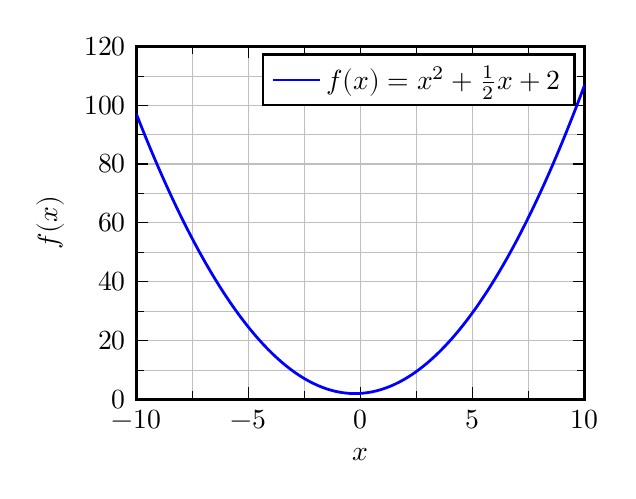
\begin{tikzpicture}
				\begin{axis}[
					width=.6\textwidth,
					height=.5\textwidth,
					domain=-10:10,
					xmin=-10, xmax=10,
					ymin=0, ymax=120,
					samples=100,
					ytick distance = 20,
					minor tick num = 1,
					%grid = both,
					%title = {\textbf{Parabelplot mit TikZ}},
					xlabel = {$x$},
					ylabel = {$f(x)$},
					legend entries = {$f(x) = x^2 + \frac{1}{2}x + 2$},
					]
					\addplot+[mark=none] {x^2 + 0.5*x + 2};
				\end{axis}
			\end{tikzpicture}
			\caption{Example plot for an expression using pgfplots}
			\label{fig:parabelpgf}
		\end{figure}
	
		Another, more advanced example is given in Figure~\ref{fig:sparameterpgf}. It uses a 2-port S-Parameter file to plot the input reflection in a smith chart and also reflection and transmission in a linear plot. The diagrams are created in a separate file using standalone. Also note that the package \texttt{subcaption} is used to create subplots.
	
		\begin{figure}[h]
			\centering
			\begin{subfigure}{0.75\textwidth}
				\centering
				\includestandalone{standalones/sparameter/sparameterSmith}
				\caption{Smith Chart plot}
			\end{subfigure}
			\\
			\begin{subfigure}{0.75\textwidth}
				\centering
				\includestandalone{standalones/sparameter/sparameter}
				\caption{}
			\end{subfigure}
			\caption{S-Parameter of a filter created on the website \url{https://rf-tools.com}}
			\label{fig:sparameterpgf}
		\end{figure}
		
		\subsubsection{Matlab plots}
		
		To avoid the use of pixel graphics there exist tools like \texttt{matlab2tikz}\footnote{\url{https://github.com/matlab2tikz/matlab2tikz}}. It is recommended to use such a tool to generate high quality plots with a consistent style. \texttt{matlab2tikz} works by generating a \texttt{tex} file from within Matlab. For detailed installation and usage it is referred to the given github repository and the Matlab FileExchange.
		
		A simple example is given below:
		
		\begin{lstlisting}[language=Matlab]
			% generate x and y data
			x=-10:0.1:10;
			y=x.^2 + 1/2*x + 2;
			
			% plotting
			figure(1);
			hold on;
			xlabel('$x$');
			ylabel('$f(x)$');
			plot(x,y,'r')
			legend('$f(x)=x^2 + \frac{1}{2}x + 2$');
			matlab2tikz('pathtotargetfile/matlabtikz.tikz', 'width', '0.5\textwidth', 'parseStrings', false);
		\end{lstlisting}
	
		When previewing graphs in Matlab axis labels appear corrupted because the {\LaTeX} commands are not interpreted in the preview due to the \texttt{parseStrings} option. 
		
		\subsubsection{Python plots using matplotlib}
		
		There are several possibilities to include python plots in {\LaTeX} documents. One of them is the \texttt{pgf} mode of \texttt{matplotlib}. It can be activated with \verb|mpl.use('pgf')| and finally the output can be saved with \verb|plt.savefig("pa2.pgf",bbox_inches='tight')| and \verb|plt.close()|. This method has the advantage that {\LaTeX} expressions inside the graphic are interpreted in the main document allowing i.e. to include cites.
		
		An alternative is \texttt{tikzplotlib} \footnote{\url{https://pypi.org/project/tikzplotlib/}} which allows a more consistent style.
		
	\subsection{Tables}
	
		There are several enhancements for {\LaTeX} tables to improve the default \texttt{tabular} environment. The \texttt{bama} class uses \texttt{longtable} for multi page tables and \texttt{booktabs} for a cleaner design. A simple example is given below:
		
		\begin{lstlisting}[language=TeX]
			\begin{table}
				\centering
				\caption{myTableCaption}
				\label{tab:myTable}
				\begin{longtable}{cc}
					\toprule
					header & second column\\
					\midrule
					content & second column\\
					next row & second column\\
					\bottomrule
				\end{longtable}
			\end{table}
		\end{lstlisting}
	
\section{Lists}

This section refers to lists like the table of contents, list of abbreviations, \dots. These are automatically generated by {\LaTeX}. In order to fully populate them several runs of the compiler may are necessary because the references have to be found in the current run but can not be processed until the next run.

The lists can be generated by the following commands. Some of them are modified by the template in order to provide the required style.

\begin{table}
	\centering
	\caption{Lists of a thesis}
	\label{tab:listofs}
	\begin{tabular}{ll}
		\toprule
		Table of contents:    & {\verb|\tableofcontents|} \\
		List of abbreviations: & {\verb|\printacronyms|} \\
		Bibliography:  & {\verb|\printbibliography|} \\
		List of figures: & {\verb|\listoffigures|} \\
		List of tables:   & {\verb|\listoftables|}\\
		\bottomrule
	\end{tabular}
\end{table}

	\subsection{Abbreviations}
	\label{sec:acronyms}

	Despite a lot of abbreviations are very common in science and engineering the long form of every abbreviation has to be included in the thesis. Therefore there is the package \texttt{acro} which offers the definition of abbreviations in separate file (\texttt{acronyms.tex}) and their use in the document.
	
	\begin{lstlisting}[language=TeX]
	\DeclareAcronym{MOSFET}{
		short = MOSFET,
		long  = Metal-Oxide-Semi\-conductor Field-Effect Tran\-sistor
	}
	\end{lstlisting}

	The abbreviation can be inserted with \verb|\ac{key}| This uses the long form at the first time like \ac{MOSFET} and the short form on the following uses like \ac{MOSFET}.
	
	Long and short forms can also be enforced using \verb|\acl| and \verb|\acs|. Beside that several commands for singular, plural, \dots are available.
	
	Used abbreviations are also included into the list of abbreviations.

	\subsection{Citations}
	\label{sec:literatur}

	Quote worthy literature is cited by the command \verb|\cite| with the literatures key as argument. The style is defined by the template and should by used for a thesis at \acs{LTE} which looks like \cite{BibDEMO1}. Cites can be inserted in the middle of sentences or at the end. Citations at the end of a sentence must be preluded by a space and directly followed by the full stop.
	
	The correct and complete citation of information from literature is absolutely mandatory. A good practice is to insert citations into the caption of figures if they are not created by the author. Referencing common knowledge like Ohm's Law is not necessary.
	
	Bibliography data is stored in bibfiles. There is an entry for every reference.
	
		\begin{verbatim}
		@Article{JassSenBigPaper,
   author  = {Hugh {Jass sen.}},
   title   = {A very-big paper},
   journal = {The journal of very big papers},
   year    = {7991},
   volume  = {MCMXCVII},
		}
		\end{verbatim}
		
		The entry is referred to by the key which is necessary for citing: \verb|\cite{JassSenBigPaper}|. Even before the key is the type of the publication like article, book, conference, online and much more. Additional information is stored according to the chosen type. Depending on the reference type the entry contains different information and looks different in the list of bibliography.
		
		Brackets are used in different places of the entry to avoid wrong wrong formatting. The example uses a bracket to declare \enquote{Jass sen.} as the last name. Otherwise {\LaTeX} would detect \enquote{sen.} as the last name which would lead to an incorrect entry in the list of bibliography.
		
		Luckily the entries rarely have to be created manually. For books the website of the university library\footnote{\url{https://ub.fau.de/}} can serve as a comprehensive source. The entries can also be obtained by the publisher. Citations for papers in electronics engineering can be mostly downloaded from \footnote{\url{https://ieeexplore.ieee.org/}}. To make the job even easier there are numerous tools for managing bibfiles. A common tool is JabRef \footnote{\url{https://www.jabref.org/}} which allows for direct imports from IEEExplore by their number. The automatic formatting generation of citekeys can also be handy. Furthermore JabRef supports the import of metadata from PDFs. Simple drag and drop can be used to import references into JabRef. The current bama template is setup to contain the necessary data.
		
		The entries should contain a unique identifier to yield a useful bibliography. This can be the ISBN for books like \cite{tietze2019} or the DOI for digital formats like \cite{paskin1999}. The corresponding url is automatically inserted as invisible link into the bibliography.
		
		Less scientific works can be described by the type \texttt{TechReport} or \texttt{online} like \cite{stm32l476, lehman2020}. These often do not contain a single author which is ok, but it has to be made sure that the reference can be found e.g. by giving a revision number.
		
		The inclusion of bibliography data is not done by {\LaTeX} itself but the a bibliography backend. In this template \texttt{biber} is used which generates a file that is included in additional runs of {\LaTeX}. This mechanism is the reason why several iterations are necessary to fully populate the bibliography.

	\section{Source Code}

		Code can be included by the environment \texttt{lstlisting}. Code can be directly inserted by the following command.
		
		\lstnewenvironment{lstlistingoflisting}
		{\lstset{language=TeX}}
		{}
		\begin{lstlistingoflisting}[language=TeX]
			\begin{lstlisting}[language=C]
				#include<stdio.h>
				
				int main(void) {
					printf("Hallo Welt"); // comment (Test for special chars: äöüß)
					return 0;
				}
			\end{lstlisting}
		\end{lstlistingoflisting}
	
		yielding

		\begin{lstlisting}[language=C]
			#include<stdio.h>

			int main(void) {
				printf("Hallo Welt"); // comment (Test for special chars: äöüß)
				return 0;
			}
  		\end{lstlisting}

		Code can also be read in form files with \texttt{firstline} and \texttt{lastline} specifying the used part of the file. \texttt{firstnumber} is the first number on the left side of the code block.
		
		\begin{lstlisting}[language=C]
			\lstinputlisting[language=C, firstline=15, lastline=17, firstnumber=15]{code/codeexample.c}
		 \end{lstlisting}
		
	\section{Indices\index{Indices}}
	
		{\LaTeX} also supports the creation of indices but it has been removed from the template due to the seldom use. It can be added with the package \texttt{imakeidx}. It supports simple indice \verb|\index{indice}| and sub-indices \verb|\index{indice!subindice}|. It is necessary to also execute \textit{makeindex} in a similar fashion than the bibliography.

	\section{Why Lua{\LaTeX}?}
	
		Lua{\LaTeX} supports additional features compared to pdflatex like direct entering of \enquote{°}, \enquote{µ} and umlaut in the code. It is also possible to execute scripts like outputting the value of $\pipi = \SI{\directlua{tex.print(math.pi)}}{}$ or the generation of PDF metadata from user variables.
		
	\section{Additional packages}
	
	Feel free to modify the files in the \texttt{header} folder to include further packages if you have additional needs like making notes with the \texttt{ToDoNotes} package which allows inserting colourful notes that can be hidden with one switch.
	
	If you have found an improvement to basic settings and packages please let the maintainer of the template know in order to improve the template.

\section{Troubleshooting}
\label{sec:troubleshooting}

	Aside from errors in the source code being one of the top reasons problems can also arise due to outdated files created by the {\LaTeX} Compiler. Deleting auxiliary files, by hand or with the function of TeXstudio, and recompiling the document can solve the problem. Further error sources are listed below.
	
	\begin{itemize}
		\item Outdated packages; {\LaTeX} packages are updated regularly. This can lead to outdated packages of the user which can be resolved by updating or the use of outdated options of the template.
		\item Missing packages; Wrong spelling of commands or using commands of not included packages lead to errors.
		\item Missing or wrong brackets
		\item Environments which do not end or are incorrectly nested.
		\item Using match commands like \verb|\frac| outside of the math mode.
		\item Tables spanning more than one page. This can resolved with the \texttt{longtable} package.
		\item Wrong format of source code files. \enquote{utf8} is recommended.
	\end{itemize}

	Further good practices are:
	\begin{itemize}
		\item Do not change files of the {\LaTeX}-installation. This avoids compilation on other machines.
		\item Do not use absolute paths. This avoids compiling the document on other machines.
	\end{itemize}

	For the most problems there is a lot of information available online. Common and also not that common problems can be found in forums but the package documentations are also pretty helpful.


	%content of the thesis splitted in several chapters
	
	%Introduction
	%
	%What is it all about?
	%Motivation, context, task definition, own approach
	% !TeX root = ../thesis.tex

\chapter{Introduction}
\label{chap:introduction}

The development of the first ECG machine in the Netherlands by Willem Einthoven marked the beginning of a revolution in monitoring cardiac activity. As of 2023, cardiovascular diseases, particularly \ac{IHD}, are among the top \ac{NCDs} , resulting in approximately 18 million deaths worldwide annually~\cite{who2023}. Cardiac arrhythmias, which include conditions such as premature ventricular and atrial contractions, \ac{AF}, ventricular fibrillation, and atrial flutter, are common and significant due to their association with increased risk of severe cardiovascular events like strokes, heart failure, and coronary artery disease~\cite{sharma2018, liu2021}. Atrial fibrillation, in particular, is a leading cause of mortality as it complicates the detection and management of cardiovascular conditions~\cite{liu2021}. \ac{ECG} play a crucial role in the diagnosis and management of arrhythmias, using waveforms to provide essential first-hand information on cardiac function under various conditions. Timely and accurate ECG monitoring is thus critical for the effective treatment of cardiovascular diseases.

\section{Motivation}

\subsection{Diagnostic Challenges and Limitations of Traditional ECG Monitoring}

Since Einthoven's pioneering work, ECG technology has undergone substantial evolution. However, the 12-lead ECG system remains the gold standard for recording cardiac waveforms. This system uses ten electrodes: six are placed on the chest (V1 to V6) and four on the limbs. Depending on the electrode combination, twelve different lead signals can be captured for diagnosing conditions such as atrial fibrillation~\cite{liu2021}. Traditionally, these 12-lead ECGs have been instrumental in diagnosing AF, requiring skilled physicians to record and interpret the results accurately. However, AF can often be asymptomatic, making it challenging to detect since symptoms may not be present during standard ECG tests~\cite{page2003}. Additionally, the intermittent nature of AF necessitates extended monitoring, which is impractical with the cumbersome 12-lead setup due to discomfort and complexity, especially for long-term wear~\cite{liu2021}. Consequently, this reliance on healthcare professionals for interpretation also delays timely intervention, making the process expensive and logistically challenging for many patients.

\subsection{The Evolution of IoT and Continuous Monitoring in Cardiac Care}

The integration of \ac{IoT} technologies in healthcare represents a significant advancement in medical monitoring. IoT-enabled ECG systems are now capable of continuously sensing cardiac signals and transmitting the raw data to cloud-based or remote servers for further analysis. This shift has the potential to automate the detection of AF using advanced machine learning algorithms, substantially reducing the time and cost associated with traditional diagnostic methods. However, these systems often rely on high-energy-consumption wireless communication technologies such as Zigbee and Bluetooth, leading to devices that are power-intensive and not ideal for continuous, long-term monitoring~\cite{muhoza2023}.

\subsection{Advancing ECG Architecture with Embedded Edge AI}

The pursuit of personalized medicine increasingly demands technologies that enable reliable, comfortable, and affordable monitoring of heart activity in everyday settings. Addressing the challenges of power consumption and patient comfort requires advancing the medical sensing architecture. Recent advancements in microcontroller capabilities and the advent of sophisticated deep learning algorithms allow for running compact AI models directly on microcontrollers~\cite{muhoza2023}. This study aims to develop a cost-effective, two-electrode (single-lead) ECG system for efficient R peak detection, which simplifies continuous monitoring. Furthermore, by leveraging edge AI technology, the system can locally process data to detect abnormalities in real time, thereby reducing power consumption and enhancing the feasibility of long-term cardiac health monitoring.

\section{Scope of the Thesis}

This thesis focuses on developing a physiological sensor board for the acquisition of ECG signals and classifying heart abnormalities at the edge. The project aims to provide a simple and cost-efficient method for acquiring ECG signals, enhancing the security and usability of ECG monitoring, and detecting abnormalities through the integration of hardware-accelerated embedded AI and a secure element. This thesis proposes a new architecture that can significantly improve medical sensing technology, making the sensing process easier, faster, and more power-efficient.

\subsection{Detailed Objectives}

\begin{itemize}
	\item \textbf{ECG System Development:} The thesis designed a compact, two-electrode ECG system optimized for user comfort and simplicity, making it suitable for long-term continuous monitoring.
	\item \textbf{Embedded AI Integration:} Embedded \ac{AI} was implemented using the Maxim78000 platform to process ECG data on-device, reducing dependency on remote processing and aiming to improve the speed and reliability of cardiac abnormality detection.
	\item \textbf{Security Implementation:} The Infineon OPTIGA Trust M secure element was utilized to ensure all patient data is encrypted, addressing the critical need for privacy and security in healthcare applications.
	\item \textbf{Energy Efficiency Analysis:} The system's power consumption was evaluated and optimized to extend battery life, which is essential for continuous monitoring applications.
\end{itemize}

\subsection{Delimitation}

The research focused on the development and initial testing of the ECG monitoring system within a lab environment and did not include commercial product development or explore the regulatory aspects of medical device approval.

\section{Outline of the Thesis}

This thesis is organized into the following chapters:

\begin{enumerate}
	\item \textbf{Chapter 1: Introduction} \\
	Introduces the research background, problem statement, objectives, and scope of the thesis.
	\item \textbf{Chapter 2: Literature Review} \\
	Reviews the physiological generation of heart signals, existing technologies, methodologies, and different architectures used in ECG monitoring. It also examines microcontrollers capable of running edge AI algorithms, comparing their energy consumption and computational capabilities, and discusses the importance of security in medical sensing.
	\item \textbf{Chapter 3: System Design and Development} \\
	Discusses the hardware and software design architecture of the complete physiological sensor board for ECG, covering everything from PCB design—including circuit design, filter design, \ac{ADC} conversion, data transfer—to component selection and integration of the Maxim78000 edge AI and Infineon secure element.
	\item \textbf{Chapter 4: Implementation and Testing} \\
	Describes the experimental setup and methodologies used for performance and security testing, detailing the implementation of the neural network on the Maxim78000 and the integration steps involved.
	\item \textbf{Chapter 5: Results and Discussion} \\
	Presents experimental results and analyzes the performance of the system in terms of energy efficiency, power consumption, and accuracy. It discusses the findings in the context of existing technologies and the theoretical framework established in earlier chapters.
	\item \textbf{Chapter 6: Conclusions and Future Work} \\
	Summarizes the research, evaluates the achievements relative to the original goals, and suggests future research directions to further enhance the system’s capabilities.
\end{enumerate}

	
	%Basics
	%
	%What do you need to know to understand the further chapters
	%All necessary information for understanding the thesis
	% !TeX root = ../thesis.tex

\ifgerman{\chapter{Grundlagen}}
\ifenglish{\chapter{Basics}}

	
	%State of the art
	%
	%What distinguishes your own approach from the state of the art?
	%Presentation and discussion of the competing solution approaches
	% !TeX root = ../thesis.tex

\ifgerman{\chapter{Stand der Technik}}
\ifenglish{\chapter{State of the art}}

	
	%Methods
	%
	%How is the approach implemented and checked?
	%All necessary information for the reproduction
	% !TeX root = ../thesis.tex

\ifgerman{\chapter{Methoden}}
\ifenglish{\chapter{Methods}}

	
	%Results
	%
	%Well, does it work?
	%Results of measurements/simulations etc.
	% !TeX root = ../thesis.tex

\ifgerman{\chapter{Ergebnisse}}
\ifenglish{\chapter{Results}}

	
	%Discussion
	%
	%How to interpret the results?
	%Discussion of successes, limitations and explanatory approaches
	%Next steps to be taken
	% !TeX root = ../thesis.tex

\ifgerman{\chapter{Diskussion}}
\ifenglish{\chapter{Discussion}}

\ifgerman{\section{Zusammenfassung}}
\ifenglish{\section{Summary}}

\ifgerman{\section{Ausblick}}
\ifenglish{\section{Outlook}}


	{\backmatter
	
	% Literatur-, Abbildungs-, Tabellenverzeichnis
	\printbibliography
	\listoffigures
	\listoftables

	%if you want to include a cv
	%\include{chapter/cv}
	}
	
	%different section numbering with letters
	\appendix
	
	%appendix content, e.g. long derivations, lots of plots, ...
	\ifgerman{\chapter{Anhang}}
\ifenglish{\chapter{Appendix}}

\section{Close view on details}


\end{document}
